\documentclass[tikz,border=5pt]{standalone}
\usepackage{luatexja}
\usepackage[hiragino-pron]{luatexja-preset}
\usepackage{amsmath,amssymb}
\usetikzlibrary{arrows.meta,patterns}

\begin{document}
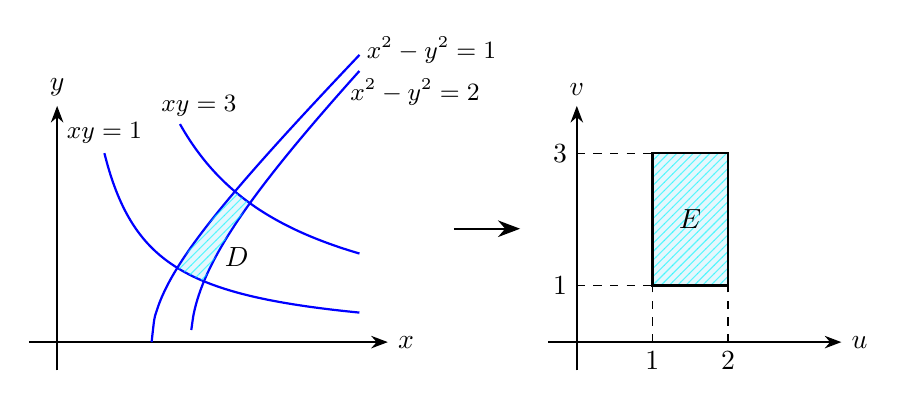
\begin{tikzpicture}[scale=1.2]

% D region (xy-plane, left)
\begin{scope}
  % Axes
  \draw[-{Stealth[length=6pt]}, thick] (-0.3,0) -- (3.5,0) node[right] {$x$};
  \draw[-{Stealth[length=6pt]}, thick] (0,-0.3) -- (0,2.5) node[above] {$y$};

  % Hyperbolas x^2 - y^2 = 1 and x^2 - y^2 = 2
  \draw[thick, blue, domain=1:3.2, samples=80, smooth] plot (\x, {sqrt(\x*\x - 1)});
  \node[right, xshift=6pt, yshift=9pt] at (3.0, {sqrt(9-1)}) {\small $x^2 - y^2 = 1$};
  \draw[thick, blue, domain=1.42:3.2, samples=80, smooth] plot (\x, {sqrt(\x*\x - 2)});
  \node[right] at (3.0, {sqrt(9-2)}) {\small $x^2 - y^2 = 2$};

  % Hyperbolas xy = 1 and xy = 3
  \draw[thick, blue, domain=0.5:3.2, samples=80, smooth] plot (\x, {1/\x});
  \node[above] at (0.5, 2.0) {\small $xy = 1$};
  \draw[thick, blue, domain=1.3:3.2, samples=80, smooth] plot (\x, {3/\x});
  \node[above, yshift=3pt] at (1.5, 2.2) {\small $xy = 3$};

  % Fill region D
  \begin{scope}
    \clip plot[domain=1:3.2, samples=80, smooth] (\x, {sqrt(\x*\x - 1)}) -- (3.2,0) -- (1,0) -- cycle;
    \clip plot[domain=1.42:3.2, samples=80, smooth] (\x, {sqrt(\x*\x - 2)}) -- (3.2,2.5) -- (0,2.5) -- (0,0) -- (1.42,0) -- cycle;
    \clip plot[domain=0.4:3.2, samples=80, smooth] (\x, {1/\x}) -- (3.2,0) -- (3.2,2.5) -- (0,2.5) -- (0,2.5) -- cycle;
    \clip plot[domain=1.0:3.2, samples=80, smooth] (\x, {3/\x}) -- (3.2,0) -- (0,0) -- (0,2.5) -- (1.0,2.5) -- cycle;
    \fill[pattern=north east lines, pattern color=cyan, opacity=0.6] (0,0) rectangle (3.5,2.5);
    \fill[cyan, opacity=0.1] (0,0) rectangle (3.5,2.5);
  \end{scope}

  % Label
  \node at (1.9,0.9) {$D$};
\end{scope}

% Arrow
\draw[-{Stealth[length=8pt]}, thick] (4.2,1.2) -- (4.9,1.2);

% E region (uv-plane, right)
\begin{scope}[shift={(5.5,0)}]
  % Axes
  \draw[-{Stealth[length=6pt]}, thick] (-0.3,0) -- (2.8,0) node[right] {$u$};
  \draw[-{Stealth[length=6pt]}, thick] (0,-0.3) -- (0,2.5) node[above] {$v$};

  % Rectangle E
  \fill[pattern=north east lines, pattern color=cyan, opacity=0.6]
    (0.8,0.6) rectangle (1.6,2.0);
  \fill[cyan, opacity=0.1]
    (0.8,0.6) rectangle (1.6,2.0);
  \draw[thick] (0.8,0.6) rectangle (1.6,2.0);

  % Dashed guides
  \draw[dashed, thin] (0.8,0) -- (0.8,0.6);
  \draw[dashed, thin] (1.6,0) -- (1.6,0.6);
  \draw[dashed, thin] (0,0.6) -- (0.8,0.6);
  \draw[dashed, thin] (0,2.0) -- (0.8,2.0);

  % Labels
  \node[below] at (0.8,0) {$1$};
  \node[below] at (1.6,0) {$2$};
  \node[left] at (0,0.6) {$1$};
  \node[left] at (0,2.0) {$3$};
  \node at (1.2,1.3) {$E$};
\end{scope}

\end{tikzpicture}
\end{document}
